\documentclass[a4paper]{book}

\usepackage[UTF8]{ctex}
\setCJKmainfont[BoldFont=SourceHanSerifSC-Bold,
                ItalicFont=KaiTi]
                {SourceHanSerifSC-Regular}

\usepackage{amsmath}

\usepackage{newtxtext,newtxmath}

% \sum
\DeclareSymbolFont{largesymbolsCM}{OMX}{cmex}{m}{n}
\let\txsum\sum
\let\sum\relax
\DeclareMathSymbol{\sum}{\mathop}{largesymbolsCM}{"50}

% \infty
\DeclareSymbolFont{symbolsCM}{OMS}{cmsy}{m}{n}
\SetSymbolFont{symbolsCM}{bold}{OMS}{cmsy}{b}{n}
\let\txinfty\infty
\DeclareMathSymbol{\infty}{\mathord}{symbolsCM}{"31}

% \partial, \pi
\DeclareSymbolFont{lettersCM}{OML}{cmm} {m}{it}
\SetSymbolFont{lettersCM}{bold}{OML}{cmm} {b}{it}
\let\txpartial\partial
\DeclareMathSymbol{\partial}{\mathord}{lettersCM}{"40}
\let\txpi\pi
\DeclareMathSymbol{\pi}{\mathord}{lettersCM}{"19}

% int 
\usepackage{esint}
\usepackage[palette=munch]{nexus}

\usepackage{tikz}
\usetikzlibrary{arrows,intersections}
\tikzset{thick,
        >=stealth',
        dot/.style={draw,circle,inner sep=0pt,minimum size=4pt}
        }

\pagestyle{empty}

\begin{document}

\definecolor{upper}{RGB}{92 172 238}
\begin{textblock}{1}(0,0)
    \noindent\textcolor{upper}{\rule{\paperwidth}{.55\paperheight}}
\end{textblock}

\begin{textblock}{1}(0,.55)
    \noindent\textcolor{black}{\rule{\paperwidth}{.45\paperheight}}
\end{textblock}

\begin{textblock}{1}(.1,.09)
    \noindent{\fontsize{28}{2}\selectfont
        \bfseries\textcolor{white}{数学之美}}
\end{textblock}

\begin{textblock}{1}(.1,.15)
    \noindent {\fontsize{22}{2}\selectfont
    \bfseries\textcolor{white}{The Beauty of Mathematics}}
\end{textblock}

\begin{textblock}{.5}(.5,.20)
\begin{center}
    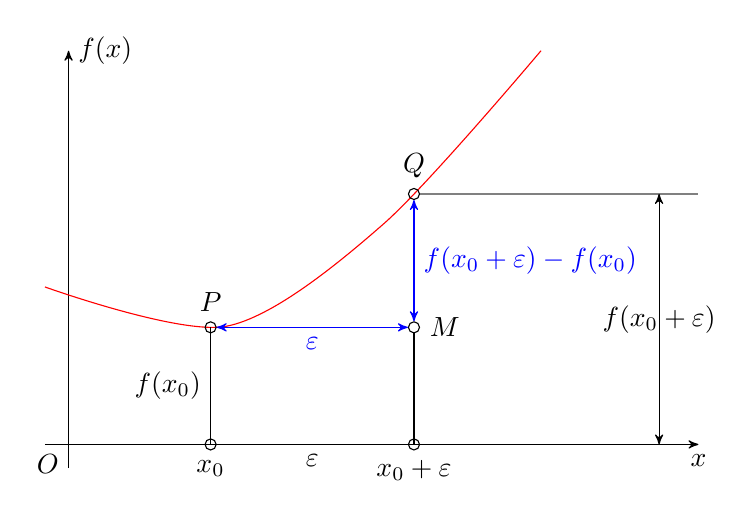
\begin{tikzpicture}
    % 画坐标系 并且定义了 O 、xmax 和 ymax
    \coordinate (O) at (0,0);
    \node [below left] at (0,0) {$O$};
    \draw[->] (-0.3,0) -- (8,0) coordinate[label={below:$x$}] (xmax);
    \draw[->] (0,-0.3) -- (0,5) coordinate[label={right:$f(x)$}] (ymax);
    % 给出直线 x 与曲线 y 的路径
    \path[name path=x] (0.3,0.5) -- (6.7,4.7);
    \path[name path=y] plot[smooth] coordinates {(-0.3,2) (2,1.5) (4,2.8) (6,5)};

    % 利用 intersections 包的计算方法,得到了直线与曲线的交点坐标,分别命名为 i-1 和 i-2 (图中分别为 P 和 Q) 过点 P 的水平线与过 Q 的竖直延长线的交点标记为 M.

    \begin{scope}[name intersections = {of= x and y,name = i}]
        % 在空白处标记 Sekante
        %\draw (0.3,0.5) -- (6.7,4.7) node[pos=0.8,below right]{};
        % 画出曲线路径 y,与之前代码几乎一样
        \draw[red] plot[smooth] coordinates {(-0.3,2) (2,1.5) (4,2.8) (6,5)};
        % 从 P 向 x 轴引垂线,垂足坐标为 (i-1 |- O),标签为 x_0
        \draw (i-1) node[dot,label={above:$P$}] (i-1) {} -- node[left] {$f(x_0)$} (i-1 |- O) node[dot,label={below:$x_0$}] {};
        % Q 点向 M 引垂线
        \path (i-2) node[dot,label={above:$Q$}] (i-2) {} -- (i-2 |- i-1) node[dot,label={right:$M$}] (i-12) {};
        % M 向 x 轴引垂线,并且标注
        \draw (i-12) -- (i-12 |- O) node[dot,label={below:$x_0 + \varepsilon$}] {};
        % 连接 Q 与 M,并且标注
        \draw[blue,<->] (i-2) -- node[right] {$f(x_0 + \varepsilon) - f(x_0)$} (i-12);
        % 连接 P 与 M
        \draw[blue,<->] (i-1) -- node[below] {$\varepsilon$} (i-12);
        % x 轴上两个垂足之间标记
        \path (i-1 |- O) -- node[below] {$\varepsilon$} (i-2 |- O);
        % Q 的水平延长线
        \draw[gray] (i-2) -- (i-2 -| xmax);
        % 标注 Q 点的垂直距离,最精彩的是用到了 xshift=-0.5cm,简直赞!
        \draw[<->] ([xshift=-0.5cm]i-2 -| xmax) -- node {$f(x_0 + \varepsilon)$}  ([xshift=-0.5cm]xmax);
    \end{scope}

    \end{tikzpicture}
\end{center}
\end{textblock}

\begin{textblock}{1}(.1,.45)
    \noindent {\fontsize{20.74}{2}\selectfont
        \bfseries\textcolor{white!80!yellow}{任\ 涛}}
\end{textblock}

\begin{textblock}{.9}(.05,.45)
    \begin{flushright}
        \noindent {\fontsize{20.74}{2}\selectfont
            \bfseries\textcolor{orange!66!red}{Version 3.14}}
    \end{flushright}
\end{textblock}

\begin{textblock}{.9}(.05,.50)
    \begin{flushright}
        \noindent {\fontsize{15}{2}\selectfont
            \bfseries\textcolor{yellow!80!cyan}{Under the LPPL, version 1.3c}}
    \end{flushright}
\end{textblock}

\begin{textblock}{.45}(.5,.56)
    \begin{center}
        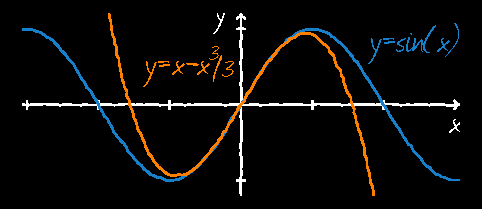
\includegraphics[width=.45\paperwidth]{dlsin}
    \end{center}
\end{textblock}

\begin{textblock}{.4}(.05,.65)
    \begin{center}
        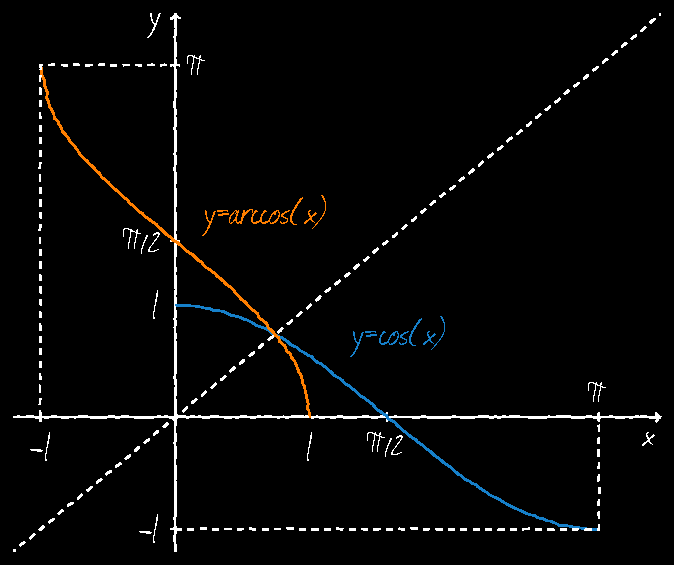
\includegraphics[width=.4\paperwidth]{arccos}
    \end{center}
\end{textblock}

\begin{textblock}{.6}(.05,.58)
    \noindent {\fontsize{20.74}{18}%
    \textcolor{white}{$\displaystyle(a+b)^n = \sum_{k=0}^n 
                \binom{n}{k} a^kb^{n-k}$}}
\end{textblock}

\begin{textblock}{.4}(.8,.80)
    \noindent {\fontsize{14.4}{18}%
    \textcolor{white!50}{$\displaystyle 
                \binom{n}{k} = \frac{n!}{k!(n-k)!}$}}
\end{textblock}

\begin{textblock}{.5}(.6,.83)
    \noindent {\fontsize{17.28}{18}%
    \textcolor{white!10}{$\displaystyle \mathrm{e}^{\mathrm{i}\pi}+1=0$}}
\end{textblock}

\begin{textblock}{1}(.04,.93)
    \noindent {\fontsize{16}{18}%
    \textcolor{white!10}{$\displaystyle 
    \iint\limits_{\Sigma}\! P(x, y, z)\, \mathrm{d} y \mathrm{d} z+Q(x, y, z)\, \mathrm{d} z \mathrm{d} x+R(x, y, z)\, \mathrm{d} x \mathrm{d} y=\iiint\limits_{\Omega}\!\left(\frac{\partial Q}{\partial x}+\frac{\partial P}{\partial y}+\frac{\partial R}{\partial z}\right) \mathrm{d} x \mathrm{d} y \mathrm{d} z $}}
\end{textblock}

\end{document}